\documentclass[a4paper,12pt]{report}
\usepackage[utf8]{inputenc}
\usepackage{times}
\usepackage{graphicx}
\usepackage{url}
\usepackage{amsmath}
\usepackage{array}
\usepackage{mathtools}
\usepackage{ifthen}
\usepackage{mathrsfs}

\oddsidemargin 0.1in		% Left margin is 1in + this value
\textwidth 5.75in		% Right margin is not set explicitly
\topmargin 0in			% Top margin is 1in + this value
\textheight 8.5in			% Bottom margin is not set explicitly
%\setlength{\columnsep}{2cm}



\iffalse
These words need to be added to the dictionary:
Ginzburg, soliton, Runge, Kutta, CGLE, Fourier, Landau
discretise
Decide whether to use non linear, non-linear, nonlinear
\fi


\iffalse
\begin{figure}[h]
\centering
\includegraphics[width=4.6in]{correlation}
\caption{A ploperature.}
\label{corr} 
\end{figure}
\fi


\iffalse
Before I submit, make sure I check that the following have updated themselves properly.
Spell Check
Contents Page
Image reference numbers
Table reference numbers
Citation numbers
\fi








\begin{document}
\begin{titlepage}
\centering
{\ \\ }
\vspace{3cm}
{\bf  \fontsize{1.35cm}{2.5cm}\selectfont Soliton Solutions of the \vspace{0.5cm} Complex Ginzburg \\\vspace{0.5cm}Landau Equation}\\
\vspace{2cm}
{\Huge By Max Proft}\\
{\Huge u5190335}
\end{titlepage}










\newcommand{\unnum}[2]{
\ifthenelse{\equal{#1}{chapter}}{\chapter*{#2}}{
\ifthenelse{\equal{#1}{section}}{\section*{#2}}{
\ifthenelse{\equal{#1}{subsection}}{\subsection*{#2}}
{\chapter*{ERROR: #2}}}}
\addcontentsline{toc}{#1}{#2} 
}%This is the exception if no case matches!!!
\tableofcontents{}
\iffalse
The order is:
Chapter
Section
Subsection
Subsubsection (not shown in contents)
\fi








\unnum{chapter}{Sections I can already write}
3.0.1, 3.0.2 - Types of solitons, both analytic and others - I will need to do the pictures later though.\\\\
4.2.3 - Relationship between DFT and FT\\\\
5.1 - Different types of machine learning\\\\


\unnum{chapter}{Abstract}
Abstract goes here.

\unnum{chapter}{Acknowledgements}
Chuck in some very cliché acknowledgements here.












\chapter{Introduction}
\section{Things to include:}
dissipative/nonconservative\\
Where do we see this happening?\cite{Ref2}\\
nonintegrable, limitations of calculating by hand, the reason for computers\\
why searching for solutions with machine learning is needed\\
\cite[pp.~215]{RefExample} 

\section{section}
Lorem ipsum dolor sit amet, consectetuer adipiscing elit.  
Etiam lobortis facilisissem.  
\subsection{subsection}
Lorem ipsum dolor sit amet, consectetuer adipiscing elit.  
Etiam lobortis facilisissem.  
\subsection{subsection 2}
Lorem ipsum dolor sit amet, consectetuer adipiscing elit.  
Etiam lobortis facilisissem.  

\section{Second Section}
 
Lorem ipsum dolor sit amet, consectetuer adipiscing elit.  
Etiam lobortis facilisissem.  













\chapter{Derivations of the CGLE}
\section{For a Quantum System}
\section{For a Classical System}












\chapter{Types of solitons}
\subsection{Analytic Solutions}

\subsection{Other Solutions}
Chaotic, but spatially localised.











\chapter{Mathematical Theory Behind Solving the CGLE}
\section{A Comparison of Different Methods}

Finite difference, what was used initially to get it all going, is bad because you do $\delta \psi / \delta x$, so over a small time period, the $\delta \psi$ term can lose several digits of precision, not good. There are a number of other ways for this to be solved though. 
\\\\
There are analytic methods when certain parameters are forced to be 0 for example ...
\\\\ 
\\\\
For the nonlinear schrodinger equation, (author) compared various methods for solving this. Other methods are EXAMPLE, and a split step fourier method. The first is better for large, slowly changing features, the second is better for sharp peaks, and the third is a good middle man, being better at both of these. 
Given the similarity between the CGLE and NLSE, this means that this should also be a reasonably good method to do this part as well. 

\section{Split Step Fourier and Runge-Kutta Method}
\subsection{Linear evolution (Fourier)}
Here we are solving the equation: 
$$\frac{d\psi}{dt}=A\frac{d^2\psi}{dx^2}+B\psi$$
Defining the fourier transform by: 
$$\hat \psi(f)=\int\limits_{-\infty}^\infty \psi(x)e^{-i2\pi x f} dx$$
By taking the fourier transform of both sides, the equation becomes:\\
$$\frac{d \hat \psi}{dt}= C(-2\pi i f)^2 D\hat \psi (f)+\hat \psi(f)= (C-D4 \pi^2 f^2) \hat \psi(f)$$
$$\implies \hat \psi_t(f) = e^{(C-D4\pi^2 f^2)t}\hat \psi_0(f)$$
And so upon inverse fourier transforming, we get the solution to this DE, where $\hat \psi_t(f)$ is the fourier transform at time $t$.
The Fourier transform can be done numerically with a discrete fourier transform, as described in a later subsection.

\subsection{Nonlinear evolution (Runge-Kutta)}
Here we are solving the equation:
$$\frac{d\psi}{dt}=C|\psi|^2\psi + D|\psi|^4\psi$$
The runga kutta method allows you to numerically solve a 1st order differential equation. which are of the form $\frac{dy}{dt}=f(t,y)$. Similar to Euler's method (which is basically just doing a derivative from first principles), except that the runge kutta method has better convergence than this. (it goes as $h^5$ as opposed to Euler's Method which is $h^2$, the backward euler formula, $h^2$, or improved euler formula which goes as $h^3$. Here $h$ is the step size. 
\\\\
The steps for doing this are as follows:
Step 1: define $f(t,y)=f(y)=C|y|^2 y  +D|y|^4 y$
Step 2: Have an initial value for $t$ and $y$, and step size and number of steps
Step 3: define the following:
$$K_1 =f(t,y)=f(y)$$
$$K_2 =f(t+0.5h,y+0.5*h*K_1)=f(y+h*K_1/2)$$
$$K_3 =f(t+0.5h,y+0.5*h*K_2)=f(y+h*K_2/2)$$
$$K_4 =f(t+h,y+h*K_3)=f(y+h*K_3)$$
Step 4: we then progress forwards $t$ and $y$ in the following way:
$$t\rightarrow t+h$$
$$y\rightarrow y+(K_1+2K_2+2K_3+K_4)*h/6$$

\iffalse


\subsection{The relationship between a Fourier Transform and a Discrete Fourier Transform}
I am pretty sure this entire section needs to be rewritten.\\
We can approximate any function with a Fourier series. (by applying periodic boundary conditions)\\
$$f(t)=\sum\limits_{-\infty}^{\infty} c_n e^{i n t}$$
Multiplying both sides by $e^{-i m t}$ and integrating from 0 to $2\pi$, and dividing by $2\pi$:
$$\frac{1}{2\pi} \int\limits_{0}^{2\pi} f(t)e^{-i m t}dt = \frac{1}{2\pi} \sum \limits_{n=-\infty}^{\infty} c_n \int\limits_{0}^{2\pi} d^{i (n-m) t} dt= c_m$$
$$\frac{1}{2\pi} \int\limits_{0}^{2\pi} f(t)e^{-i m t}dt =c_m$$
We use the substitution:
$$t = \frac{2\pi}{L}  x \implies x = \frac{L}{2\pi} t$$
$$dt = \frac{2\pi}{L}  dx$$
And then this becomes:
$$c_m = \frac{1}{L} \int\limits_{0}^{L} f(x) e^{-i m 2\pi x/L} dx $$

For a fourier series $\{c_n\}$, the fourier transform is given given by:

$$\hat f (freq) = \sum\limits_{-\infty}^{\infty} c_n \mathscr{\hat F}(e^{i n 2 \pi x/L})(freq)$$ 

But we have $$\mathscr{\hat F}(e^{i n 2 \pi x/L}) = \int\limits_{-\infty}^\infty e^{i n 2 \pi x/L}e^{-i 2\pi freq x} dx $$
$$= \int\limits_{-\infty}^\infty e^{i x (n 2 \pi /L - 2\pi freq )}dx = 2\pi \delta (n 2\pi/L -2\pi freq)= \delta (n /L - freq)$$

And so we get:
$$\hat f (freq) = \sum\limits_{-\infty}^{\infty} c_n \delta(freq.- n/L)$$
$$= \sum\limits_{-\infty}^{\infty} c_n /L \delta(freq. L- n)$$

If we inverse fourier transform we get the following.
We can also use $x/L=n/N$
$$Data = spacial,  Fata=frequency$$


I don’t think the following is useful:
$$f(x)= \sum\limits_{n=-\infty}^\infty f_n e^{2\pi i n x/L} $$
If we multiply both sides by $e^{-2\pi i m x/L}$ and integrate we get:
$$\int \limits_{-\infty}^\infty f(x)e^{2\pi i n x/L} dx = \sum\limits_{n=-\infty}^\infty  f_n  \int \limits_{-\infty}^\infty  e^{i 2 \pi x/L (n-m)} dx  =  \sum\limits_{n=-\infty}^\infty  f_n  \int \limits_{-\infty}^\infty  e^{i 2 \pi x (n-m)/L} dx  $$
$$=  \sum\limits_{n=-\infty}^\infty  f_n \delta((n-m)/L) = f_n \delta((n-m)/L)$$

\fi




\subsection{The relationship between a Fourier Transform and a Discrete Fourier Transform:}
Below works for periodic boundary conditions, or if you assume that the function goes to zero at the boundary. For ease of proving the relationship, we assume the latter. 
\\\\
Defining the Fourier transform as:
$$\tilde \psi(f) = \int_{-\infty}^\infty \psi(x) e^{-i2\pi xf} dx \approx \int_0^L\psi(x)e^{-i2\pi x f}dx$$
Let $\Delta x=L/N$ for some integer $N$.
$$\approx \sum\limits_{n=0}^{N-1}\psi(n \Delta x) e^{-i 2\pi n \Delta x f}\Delta x$$
With the same arguments, we get the inverse Fourier transform to be:\\ 
($\Delta f = (f_1-f_0)/N$, for some values of $f_1$ and $f_2$)
$$\psi(x) = \int_{-\infty}^\infty \tilde\psi(f)e^{i 2\pi x f} df \approx \int_{f_0}^{f_1}\tilde\psi(f)e^{i 2\pi x f}df \approx \sum\limits_{m=0}^{N-1}\tilde\psi(f_0+m\Delta f)e^{i 2\pi n\Delta x f_0} e^{i 2\pi x m\Delta f}\Delta f$$
Let $\psi(n\Delta x) = \psi_n$ and $\tilde\psi(f_0+m\Delta f) = \tilde \psi_m$ and let $f_0=-\pi/\Delta x$ 
$$\tilde \psi_m\approx \Delta x \sum\limits_{n=0}^{N-1}\psi_n e^{-i 2\pi n \Delta x f_0}e^{-i 2\pi n m \Delta x \Delta f}$$
$$\psi_n  \approx \Delta f e^{i 2\pi n\Delta x f_0}\sum\limits_{m=0}^{N-1}\tilde\psi_m e^{i 2\pi n m \Delta x \Delta f}$$
Since the definition of the discrete Fourier transform is
$$\tilde A_m =  \sum\limits_{n=0}^{N-1} A_n e^{-i 2\pi n m/N}$$
$$A_n  = \frac{1}{N}\sum\limits_{m=0}^{N-1}\tilde A_m e^{i 2\pi n m/N}$$
We now have a way to compute (inverse) Fourier transforms given a set of data that is a sufficiently good approximation of the initial function.
\\\\
We want $f_1-f_0=1/\Delta x$ so that the frequency difference corresponds to the difference between adjacent elements. This means we get $\Delta f = 1/(N\Delta x)$. We then choose to take $f_0=\frac{-1}{2\Delta x}$ is chosen so it satisfies the Nyquist limit.
$$\tilde \psi_m\approx \Delta x \sum\limits_{n=0}^{N-1}\psi_n e^{i \pi n }e^{-i 2\pi n m/N}$$
$$\psi_n  \approx \frac{e^{-i \pi n}}{N\Delta x}\sum\limits_{m=0}^{N-1}\tilde\psi_m e^{i 2\pi n m/N}$$


Check I have done this the same way in my program. and that I have used $e^{i\pi n}=\pm 1$


\subsection{Combining these operations}
With the split step fourier method, we assume that the linear and nonlinear terms do not affect each other over short timescales. This means that we can propegate forwards according to the linear evolution equation, and then propegate forwards according to the nonlinear evolution equation, and we should get a good approximation for the solution to the original differential equation. This can be represented as the following, where $\hat N$ refers to the nonlinear evolution operator, and $\hat L$ refers to the linear evolution operator.
$$\psi(t)=e^{\hat N(t)}e^{\hat L(t)}\psi(0)$$ 
It turns out, however, that a more stable way of doing this evolution is with the following (notice that the two outside terms are both evolution operators for half of the time period):
$$\psi(t)=e^{\hat N(t/2)}e^{\hat L(t)}e^{\hat N(t/2)}\psi(0)$$ 




\section{Testing the Code}
\subsection{Comparison with Analytic Solutions}
Find exact solutions (to both CGLE and NLSE), and show that it matches well.
After $x$ amount of time, how accurate is the answer
\subsection{Decreasing the step size and Determining Appropriate Values}
Find interesting solitons and show that we can reproduce these solutions.\\\\
For unusual, and non-analytic solutions, especially spiny solitons, as you decrease the step size, after a length of time $t$, how close is the answer to the limit? I.e. make the time step size 0.1, and propagate forwards in time until t=10. repeat with step sizes 0.01, 0.001 and plot the final answer. It should approach a constant value. Take the step size to be the smallest value such that the solution is within 1\% of the answer with the previous step size.















\chapter{Machine Learning Theory}
\section{Different Types of Machine Learning}
I want to enter in an image, and get it to tell me if it is oscillating/etc.\\
I want another machine learning algorithm to predict the required precision, and wait time before recording the output.\\
Monte Carlo and gradient descent to find new solns.\\
\section{Linear Regression}
Former Title: Different Options for the Machine Learning Algorithm\\
Another Title Removed: A detailed look at neural networks\\
\\
Step 1: Define a cost function:\\
Suppose we have input parameters $\vec x_i$ with the true value given by $y_i$. For linear regression, we choose $\vec\theta$ such that our prediction for the value of $y_i$ is $\vec\theta \cdot \vec x_i$. We want to vary the vector $\vec \theta$ such that the predictions match as best as possible. This is typically done by providing a cost function that is lowest when the predictions match the true value best. A typical cost function is (least squares):
$$J_\theta = \sum_i \left(\vec\theta\cdot \vec x_i -y_i\right)^2 $$
\\
Suppose we have two parameters, we might get an image as shown below. 
\begin{figure}[h]
\centering
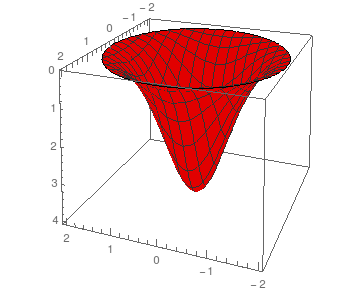
\includegraphics[width=3in]{GradDescent}
\caption{Gradient descent example}
\label{corr} 
\end{figure}
The minimum of this graph give $\theta$ which causes the best predictions. 
Typically the algorithm to find the minimum is done by continually taking the steepest path. However the algorithm may end up finding a local minima, as in the subsequent figure. 
\begin{figure}[h]
\centering
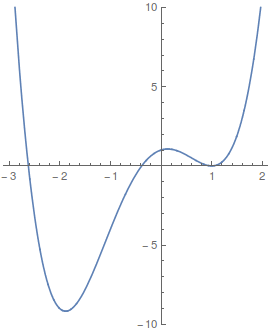
\includegraphics[width=2in]{localmin}
\caption{Gradient descent example}
\label{corr} 
\end{figure}
Octave has lots of fancy functions that can do this really efficiently, and can try to avoid local minima.
\\\\
We can increase the number of input features. One feature we want to add is an intercept term, which will equal $1$ for every training example. Other features we might want to add, for example, would be the polynomial features $\{x_1^2,x_1x_2,x_1x_3, ... \}$. However if we add in these extra features, we are faced with another issue, and that is overfitting. If we have a high degree polynomial, it becomes much easier to overfit the data. In order to prevent this, we can adjust the cost function to:
$$J_\theta = \frac{1}{2m}\sum_i \left(\vec\theta\cdot \vec x_i -y_i\right)^2 +\frac{\lambda}{2m} |\vec\theta|^2$$
By doing this, if several of the elements of $\vec \theta$ are large, then the cost will increase, and so only the important features will remain large. However for this to work we must normalise the data, and in my program this is done by transforming each feature $x_i^{(j)}$  in the following manner, where the $i$ indicates that it is the $i^{th}$ training example, and the $j$ index refers to the $j^{th}$ component of the vector. Below $\mu^{(j)}$ refers to the mean of the $j^{th}$ component of all the training examples, and $\sigma^{(j)}$ the standard deviation
$$x_i^{(j)}\rightarrow \frac{x_i^{(j)}-\mu^{(j)}}{\sigma^{(j)}}$$
This ensures that all of the features are on the same scale, and so the elements of $\theta$ are penalised equally by the cost function. 



\section{Training and Testing the Algorithm}

Tried initially with only linear terms, then expanded to polynomial terms with regularisation and it was able to fit data with polynomial features $(0.5x_1+x_2^3)$. This game me the confidence that the algorithm was working correctly, and so I could go ahead and train the algorithm on real data with confidence.\\\\
My algorithm went up to 4th order polynomial terms, and with 6 different parameters being varied, this results in a total of 210 features. 










\chapter{The result from much work}
\section{The sorts of things that I found}












\unnum{chapter}{Conclusion}
\unnum{chapter}{Appendix A}
\unnum{chapter}{Appendix B}

\begin{thebibliography}{9}
%Introduction
\bibitem{RefExample}
    Name \emph{Title},
    Publishing info, etc
\bibitem{Ref2}
    Another Guy \emph{title2}
    pub,etc.
%Derivation of CGLE

%Types of Solitons

%Mathematical theory behind solving CGLE

%Machine Learning

%My solitons


\end{thebibliography}


\end{document}